\chapter{Traballo Realizado}
\label{chap:Traballo Realizado}

\lettrine{N}{este} apartado presentarase o traballo realizado, comezando por unha vista xeral do proceso, 
seguido dunha explicación dos diferentes módulos desenvolvidos e a súa interacción, así como os conxuntos de datos empregados.
Finalmente, presentaranse os resultados obtidos acompañados dunha análise dos mesmos.
\section{Vista Xeral}
\label{sec:VistaXeral}

O proxecto consiste en adaptar o framework de IDIR, ideado para o rexistro de \gls{4DCT} torácicas, para o rexistro de imaxes de fondo de ollo en 2D.
Para isto foi necesario modificar gran parte do código, así como adaptar o proceso de rexistro e avaliación.

Inicialmente replicáronse os resultados obtidos por Wolterink et al. \cite{wolterink2021implicit} que se mostran na táboa seguinte:

\begin{table}[ht]
    \centering
    \caption{Replicación dos resultados de IDIR}
    \begin{tabular}{c|c}
        Scan & {IDIR / Replicación} \\
        1  & 0.76 (0.94) / 0.79 (0.92) \\
        2  & 0.76 (0.94) / 0.71 (0.89) \\
        3  & 0.94 (1.02) / 0.95 (1.01) \\
        4  & 1.32 (1.27) / 1.32 (1.22) \\
        5  & 1.23 (1.47) / 1.23 (1.46) \\
        6  & 1.09 (1.03) / 1.15 (1.04) \\
        7  & 1.12 (1.00) / 1.11 (0.99) \\
        8  & 1.21 (1.29) / 1.20 (1.28) \\
        9  & 1.22 (0.95) / 1.16 (0.99) \\
        10 & 1.01 (1.05) / 1.09 (1.05) \\
        Promedio & 1.07 / 1.07 (1.08) \\
    \end{tabular}
    \label{tab:comparison}
\end{table}

\FloatBarrier


\section{IDIR}
\label{sec:IDIR}
IDIR (Implicit Deformable Image Registration) é un método de aliñamento de imaxes baseado en redes neuronais. 
A súa principal diferenza frente a unha rede convolucional tradicional é que, 
en lugar de predicir a transformación entre imaxes, optimízase unha rede para esta mesma represente esta transformación.

O que \cite{wolterink2021implicit} propón é optimizar directamente o DFV facendo uso
 dunha representación implícita, de forma que a deformación está representada nos propios pesos dunha MLP.

 \cite{sun2024medicalimageregistrationneural} e \cite{nodeo} propuxeron métodos de rexistro de imaxes similares de forma independente,
 baseados en Neural ODE (ODE-Nets)\cite{neuralode}, unha familia de modelos de aprendizaxe profundo que trata a rede como un sistema continuo en lugar de unha secuencia de capas discretas.


\subsubsection{Arquitectura}
\label{subsubsec:Arquitectura}

Faise uso dun MLP de 3 capas, e determinaron experimentalmente que obtiñan mellor resultado con 256 unidades por capa que 128.
Por cada epoch de entrenamento (2500 en total), 10000 puntos son muestreados aleatoriamente do espazo de coordenadas dentro da máscara.
O término de perda é a 'normalized cross-correlation' entre os valores dos píxeles muestreados na imaxe fixa e os correspondentes da imaxe móbil.
Utilizan Adam de optimizador, cun learning rate de 0.0001.

\subsubsection{Función de activación}
\label{subsubsec:Función de activación}

Unha elección estándar para a función de activación é \textbf{ReLU}:

\[
f(x) = \max(0, x) = \begin{cases} 
x & \text{si } x > 0 \\ 
0 & \text{si } x \leq 0 
\end{cases}
\]

Non obstante, para redes de representación implícita como ca que estamos traballando, esta ten unha serie de desventaxas.

As ReLUs teñen un sesgo cara a sinais de baixa frecuencia \cite{rahaman2019spectralbiasneuralnetworks}, 
 o que significa que o modelo pode ter dificultades para representar pequenas deformacións locais no rexistro de imaxes.
 
\cite{ziyin2020neuralnetworksfaillearn} demostraron que a gran parte das funcións de activación utilizadas en redes neuronais (ReLU, tanh, sigmoide e todas as súas variantes)
son incapaces de extrapolar función periódicas sinxelas debido á súa tendencia a converxer cara a comportamentos lineais cando se extrapolan fóra do rango de adestramento. 

Existen varias formas de superar este sesgo, como preprocesar as coordenadas de entrada con funcións de activación periódicas \cite{mildenhall2020nerfrepresentingscenesneural} 
ou substituír a función de activación ReLU por unha función de activación periódica \cite{sitzmann2020implicitneuralrepresentationsperiodic}.

Neste traballo escollemos a segunda opción, utilizando unha función de activación periódica de tipo \textbf{SIREN}:

\[
f(x) = \sin(ax + b), \quad \text{con} \quad a, b \in \mathbb{R}
\]

Unha vantaxe engadida das funcións de activación periódicas nas redes SIREN é que poden ser diferenciadas varias veces, 
o que expande substancialmente o conxunto de termos de regularización que se poden empregar na rede, como veremos na seguinte sección.

larger frequencies appear in the networks for weights with larger magnitudes.

Outros traballos como \cite{mildenhall2020nerfrepresentingscenesneural} non utiliza unha función de activación periódica, mais para a representación adecuada de zonas de alta frecuencia 
utilizaron codificación posicional, que xa as incorpora de forma implícita na rede con bós resultados. 

Outra das vantaxes que ten SIREN é que é unha función suave ou infinitamente diferenciable, é dicir, que admite derivadas de calquer orde.
Outros exemplos de funcións de activación infinitamente diferenciables son:

Sigmoide:  
\[
f(x) = \frac{1}{1 + e^{-x}}
\]
Tangente Hiperbólica:  
\[
f(x) = \tanh(x) = \frac{e^x - e^{-x}}{e^x + e^{-x}}
\]

Softplus:  
\[
f(x) = \ln(1 + e^x)
\]


\paragraph{Inicialización de pesos}

En \cite{sitzmann2020implicitneuralrepresentationsperiodic} propuxeron unha inicialización específica para as redes SIREN, 
a cal consiste en inicializar a primeira capa de xeito que a función seno recorra múltiples períodos sobre o intervalo [−1,1][−1,1].
Isto conséguese multiplicando os pesos da primeira capa por un factor de escala ω0, sobre o cal recomendan ω0=30.
A fórmula para a inicialización dos pesos da primeira capa é a seguinte:

\begin{figure}[ht!]
    \centering
    \[
    w_i \sim U\left[ -\frac{1}{n}, \frac{1}{n} \right]
    \]

\caption{Inicialización primera capa}
\end{figure}

onde n é o número de neuronas de entrada (o tamaño da capa anterior).

As seguintes capas inicialízanse da seguinte forma:
\begin{figure}[ht!]
    \centering
    \[
    w_i \sim U\left[ -\frac{\sqrt{\frac{6}{n}}}{w}, \frac{\sqrt{\frac{6}{n}}}{w} \right]
    \]
    \caption{Inicialización seguintes capas}
\end{figure}

Desta forma asegurase que a entrada a cada activación sinusoidal está distribuída normalmente cunha desviación estándar de 1,
 o que debería mellorar a estabilidade e converxencia durante o adestramento da rede.
Unha consecuencia desto é que, xa que os propios pesos da rede representan a deformación, inicialmente a rede comeza cunha deformacion moi similar en todos os casos, que o entrenamento deberá corrixir.

En \cite{sireninit} implementan unha versión simplificada de SIREN para facilitar o estudo destas, 
e propoñen melloras proceso de inicialización. Unha delas e utilizar a distribución Kaiming (He) en lugar da uniforme.
Tamén propoñen un método para escoller un valor de w apropiado según o problema a resolver.

\subsubsection{Termos de loss}
\label{subsubsec:Termos de loss}

O termo de perda é a función que se optimiza durante o adestramento, e é o que guía a rede cara a unha solución óptima.
Esta cuantifica a discrepancia entre a saída da rede e o resultado desexado.

Para a tarefa de rexistro de imaxes, utilízanse dúas categorías principais de métricas para avaliar o aliñamento entre imaxes: 
as métricas baseadas no erro e as métricas baseadas na similitude. As métricas baseadas no erro (MSE, L1...) miden as diferenzas píxel a píxel entre as imaxes, 
sendo máis sensibles a diferenzas locais e proporcionando unha medida absoluta. 
As métricas baseadas na similitude (NCC, SSIM...) teñen en conta patróns estructurais e relacións estatísticas entre as imaxes, sendo máis robustas fronte a variacións na iluminación e pequenos desprazamentos.
\cite{simmetric}

Os principais termos de perda valorados para este traballo son:

\begin{itemize}
    % Error-based metrics
    \item \textbf{MSE (Mean Squared Error)}:
    Erro cadrático promedio entre á imaxe fixa e a móbil. É sensible a valores atípicos e ruido.
    \[
    \text{MSE} = \mathbb{E}[(Y - \hat{Y})^2] = \frac{1}{N} \sum_{i=1}^{N} (y_i - \hat{y}_i)^2
    \]
    onde \( y_i \) é o valor do pixel da imaxe fixa, \( \hat{y}_i \) é o valor do pixel da imaxe móbil, e \( N \) é o número total de píxeles. \cite{Palubinskas02012017}

    Regulizador Hiperelástico en 2D   \item \textbf{L1 (Mean Absolute Error)}:
    Mide o error absoluto promedio. Menos sensible a valores atípicos que MSE.
    \[
    \text{L1} = \mathbb{E}[|Y - \hat{Y}|] = \frac{1}{N} \sum_{i=1}^{N} |y_i - \hat{y}_i|
    \]

    % Robust error metrics
    \item \textbf{Huber Loss}:
    Combina MSE e L1, sendo cadrática para errores pequenos e lineal para errores grandes.
    \[
    \text{Huber}(y, \hat{y}) = \begin{cases}
    \frac{1}{2}(y - \hat{y})^2 & \text{se } |y - \hat{y}| \leq \delta \\
    \delta(|y - \hat{y}| - \frac{1}{2}\delta) & \text{noutro caso}
    \end{cases}
    \]
    onde \( \delta \) é un hiperparámetro que define o punto de transición entre os comportamentos cadrático e lineal.

    \item \textbf{Smooth L1 Loss}:
    Similar a Huber Loss, pero cunha transición suave entre as rexións cadrática e lineal.
    \[
    \text{SmoothL1}(y, \hat{y}) = \begin{cases}
    \frac{1}{2}(y - \hat{y})^2 & \text{se } |y - \hat{y}| \leq 1 \\
    |y - \hat{y}| - \frac{1}{2} & \text{noutro caso}
    \end{cases}
    \]

    % Similarity-based metrics
    \item \textbf{NCC (Normalized Cross-Correlation)}:
    Evalúa a similitude entre as dúas imaxes normalizando as súas intensidades. É invariante a cambios na iluminación.
    \[
    \text{NCC} = \frac{\sum_{i=1}^{N} (y_i - \mu_y)(\hat{y}_i - \mu_{\hat{y}})}{\sqrt{\sum_{i=1}^{N} (y_i - \mu_y)^2 \sum_{i=1}^{N} (\hat{y}_i - \mu_{\hat{y}})^2}}
    \]
    onde \( \mu_y \) e \( \mu_{\hat{y}} \) son as medias das imaxes fixa e móbil, respectivamente.

    \item \textbf{SSIM (Structural Similarity Index)}:
    Evalúa a similitude estructural entre as dúas imaxes, considerando luminancia, contraste e estructura.
    \[
    \text{SSIM}(y, \hat{y}) = \frac{(2\mu_y\mu_{\hat{y}} + C_1)(2\sigma_{y\hat{y}} + C_2)}{(\mu_y^2 + \mu_{\hat{y}}^2 + C_1)(\sigma_y^2 + \sigma_{\hat{y}}^2 + C_2)}
    \]
    onde \( \mu_y \), \( \mu_{\hat{y}} \) son as medias, \( \sigma_y \), \( \sigma_{\hat{y}} \) son as desviacións estándar, \( \sigma_{y\hat{y}} \) é a covarianza, e \( C_1 \), \( C_2 \) son constantes para evitar divisións entre cero. \cite{Palubinskas02012017}
\end{itemize}

Debido á natureza das imaxes de retina, onde poden existir diferencias de iluminación e contraste entre as imaxes fixa e móbil, 
parece mais apropiado empregar métricas baseadas na similitude como NCC ou SSIM.

NCC utilizouse a implementación de  https://github.com/BDdeVos/TorchIR/blob/main/torchir/metrics.py.

\subsubsection{Termos de regularización}
\label{subsubsec:Termos de regularización}

Debido a que o rexistro de imáxenes deformables é un problema mal planteado (ill-posed problem**), 
é común utilizar algún tipo de regularización sobre o DVF para evitar deformacións pouco realistas.
 Os métodos de rexistro baseados en redes neuronaies convolucionais (CNN) representan os DVFs
 como mostras en una cuadrícula de vóxeles, e polo tanto, solo se poden aproximar gradientes espaciais
 mediante esquemas de diferencias finitas (aproximar derivadas mediante cálculo numérico de diferencias entre valores adyacentes en la cuadrícula).
 Este é un proceso computacionalmente moi costoso e ineficiente, ademais implica errores de discretización e perdas de precisión.


Facendo uso de representacións implícitas, todas as operación son diferenciables, e os gradientes poden
 ser computados facilemente de forma analítica en lugar de ter que aproximalos, facendo uso da librearía de autodiferenciación de PyTorch.

Utilizando ReLU como función de activación, a rede é diferenciable unha vez, mentres que utilizando
 unha función de activación periódica (como SIREN), a rede é diferenciable todas as veces que se precise.
Desta forma, podemos calcular calquera número de termos de regularización e incluilos na optimización da rede.

Algúns exemplos de termos de regularización que se poden empregar son:
\begin{itemize}
    \item Jacobian regularizer: 
    O determinante Jacobiano da transformación (det ∇Φ) nunha localización x é un indicador de estiramento ou compresión local.
    Un determinante Jacobiano negativo ou moi cercano a 0 indica que están a ocurrir dobreces e a transformación non será invertible.
    A matriz jacobiana é a matriz que contén todas as derivadas parciais da función de transformación (calculado mediante gradientes).
    O termo de regularización do Jacobiano penaliza os valores do determinante Jacobiano que se desvían de 1, 
    tentando preservar áreas locais e evitar estiramentos ou dobreces extremas.


    \begin{figure}[ht!]
        \centering
        \[
        S^{jac}[\Phi] = \int_{\Omega} \left| 1 - \det \left( \nabla \Phi \right) \right| \, dx
        \]
        \caption{Regulizador Jacobiano}
    \end{figure}

    Ω representa o dominio ou rexión do espazo sobre o cal está definida a transformación Φ.
    
    \item Hyperelastic regularizer
    Tamén se póden engadir restricións ao DVF con este termo proposto por \cite{HyperelasticRegularization}.
    Consiste en tres termos, un termo de lonxitude, un termo de área e un termo de volumen co obxetivo de controlar variacións nestes aspectos.
    O termo de lonxitude penaliza a variación da lonxitude dos vectores do DVF, sendo u a medida desplazamiento dun punto no espacio.
    A matriz de cofactores da matriz do Jacobiano da transformación controla o área, 
    A función de máximo asegura que só as expansións que sobrepasen certo límite sexan penalizadas
    O determinante da matriz do Jacobiana controla o volume, 
    e ambas penalizan o crecemento e a contracción por igual.
    αl, αa e αν son hiperparámetros que controlan a importancia de cada término.

    \begin{figure}[ht!]
        \centering
        \[
        S^{hyper}[\Phi] = \int_{\Omega} \left[ \frac{1}{2} \alpha_1 |\nabla u|^2 + \alpha_a \varphi_c (\text{cof} \nabla \Phi) + \alpha_\nu \psi(\det \nabla \Phi) \right] dx,
        \]
        \[
        \text{Funcións convexas:} \quad \varphi_c(C) = \sum_{i=1}^3 \max \left\{ \sum_{j=1}^3 C_{ji}^2 - 1, 0 \right\}^2 \quad \text{and} \quad \psi(v) = \frac{(v-1)^4}{v^2}.
        \]
        \caption{Regulizador Hiperelástico.}
    \end{figure}


    \item Bending energy penalty
    Pódese impoñer a suavidade da deformación empregando esta penalización proposta en \cite{bendingenergy}, que 
    require que as segundas derivadas do DVF sexan pequenas en todo o dominio, o que evita deformacións bruscas e discontinuas.
    Este termo non pode ser utilizado nunha rede que utilice ReLU como función de activación, xa que a segunda derivada de unha ReLU é sempre igual a 0.

    \begin{figure}[ht!]
        \centering
        \[
        S^{bending}[\Phi] = \frac{1}{8} \int_{-1}^{1} \int_{-1}^{1} \int_{-1}^{1} \left[ \left( \frac{\partial^2 \Phi}{\partial x^2} \right)^2 + \left( \frac{\partial^2 \Phi}{\partial y^2} \right)^2 + \left( \frac{\partial^2 \Phi}{\partial z^2} \right)^2 \right.
        \]
        \[
        \left. + 2 \left( \frac{\partial^2 \Phi}{\partial x \partial y} \right)^2 + 2 \left( \frac{\partial^2 \Phi}{\partial x \partial z} \right)^2 + 2 \left( \frac{\partial^2 \Phi}{\partial y \partial z} \right)^2 \right] dx\,dy\,dz
        \]
        \caption{Regulizador Bending Energy}
    \end{figure}
    
\end{itemize}

Para a implementación neste traballo modificaronse todos estos termos para que funcionaran con transfomacións de dúas dimensións en lugar de tres,
 sustituíndo o gradiente de 3 dimensión no Jacobiano por un de dúas, eliminando as derivadas parciais en z en bending energy e o termo de volume no termo hiperelástico.

 \begin{itemize}
    \item Jacobian regularizer:
    \begin{figure}[ht!]
        \centering
        \[
        S^{jac}[\Phi] = \int_{\Omega} \left| 1 - \det \left( \nabla \Phi \right) \right| \, dx \, dy
        \]
        \caption{Regulizador Jacobiano en 2D}
    \end{figure}
    
    \item Hyperelastic regularizer:
    \begin{figure}[ht!]
        \centering
        \[
        S^{hyper}[\Phi] = \int_{\Omega} \left[ \frac{1}{2} \alpha_1 |\nabla u|^2 + \alpha_a \varphi_c (\text{cof} \nabla \Phi) \right] dx \, dy,
        \]
        \[
        \varphi_c(C) = \sum_{i=1}^2 \max \left\{ \sum_{j=1}^2 C_{ji}^2 - 1, 0 \right\}^2
        \]
        \caption{Regulizador Hiperelástico en 2D}
    \end{figure}
    
    \item Bending energy penalty:
    \begin{figure}[ht!]
        \centering
        \[
        S^{bending}[\Phi] = \frac{1}{8} \int_{-1}^{1} \int_{-1}^{1} \left[ \left( \frac{\partial^2 \Phi}{\partial x^2} \right)^2 + \left( \frac{\partial^2 \Phi}{\partial y^2} \right)^2 + 2 \left( \frac{\partial^2 \Phi}{\partial x \partial y} \right)^2 \right] dx \, dy
        \]
        \caption{Regulizador Bending Energy en 2D}
    \end{figure}
    
\end{itemize}

A regularización tamén ten un impacto significativo no tempo de computación, xa que require múltiples pasadas de retropropagación por época para calcular os distintos termos de penalización.
Sen regularización só se fai 1 pasada para calcular o gradiente do termo de similitude da imaxe.
Ca regularización do Jacobiano, ademais do termo de similitude, calcúlanse dúas derivadas (unha por dimensión) para obter o Jacobiano, resultando en 3 pasadas por época.
Engadindo a regularización hiperelástica (sen termo de volume), é necesario calcular unha derivada adicional para o cofactor da matriz Jacobiana, facendo un total de 4 pasadas por época.
Finalmente, ca penalización de enerxía de flexión, necesitanse derivadas segundas, o que implica 7 pasadas por época en total.
No traballo orixinal de IDIR, chegaban a usar 13 pasadas debido a que traballan en 3D.

Se os termos de regularización teñen demasiada influencia sobre o termo de loss, a rede fará transformacións moi pequenas para evitar ser penalizada, o que resultará nunha transformación insuficiente.
Por outro lado, se os termos son demasiado pequenos, a rede fará transformacións moi grandes, o que resulta nunha transformación irrealista e sobreaxustada. Isto é especialmente evidente no caso da función de activación SIREN, que tende a sobreaxustarse facilmente debido ao seu sesgo cara sinais de alta frecuencia.
A cantidade óptima de regularización depende da parexa concreta de imaxes a alinear, polo que intentaremos determinar cal é a mellor para unha mostra de imaxes.

Ademais, pese a que os diferentes termos de regularización valoran diferentes aspectos, cabe ter en conta que tamén superposición nalgunhas das propiedades que valoran.
Por exemplo, o regularizador hiperelástico pode considerarse un termo mais xeral que inclúe indirectamente penalizaciones do Jacobiano (ambos penalizan as "dobreces") e de suavidade das transfomacións (como fai o bending pero en menor grado).

\subsubsection{Learning rate e batch size}
\label{subsubsec:Learning rate e batch size}

O learning rate é un parámetro do optimizador (Adam neste caso) que regula o tamaño dos axustes efectuados aos parámetros do modelo durante cada iteración de actualización. 
Determina a magnitude do cambio aplicado para minimizar a función de perda, afectando tanto a velocidade de converxencia como a estabilidade do proceso de aprendizaxe.
Un learning rate demasiado alto pode provocar que a rede diverxa, mentres que un learning rate demasiado baixo pode resultar en converxencia lenta ou quedar atrapado en mínimos locais.

Debido á natureza da rede, o batch size utilzado ten unha relación directa co learning rate, polo que tentaremos determinar a relación óptima entre ambos.

Unha das heurísiticas mais comúns para relacionar o learning rate e o batch size é a regla de escalado linear \cite{goyal2018accuratelargeminibatchsgd}. 
A regla indica que o learning rate óptimo debe escalarse linearmente co tamaño do batch size. 

Unha forma de explicar isto é, xa que con batches mais grandes temos unha mellor aproximación do gradiente real, é posible utilizar un learning rate maior sen que a rede diverxa. \cite{kexuefm}


O batch size nesta rede representa o número de coordenadas amostradas aleatoriamente do espazo de coordenadas dentro da máscara.


\subsubsection{Método}
\label{subsubsec:Método}

Sendo o obxetivo encontrar unha transformación espacial óptima entre a imaxe móbil e a imaxe fixa,
é necesario obter a función de deformación  Φ(x) = u(x) + x que mapea cada coordenada x na imaxe móbil a unha coordenada na imaxe fixa, 
de forma que a coordenada x na imaxe fixa corresponda anatomicamente á coordenada Φ(x) na imaxe móbil.
Este problema pode ser formulado como un problema de optimización onde $L_{data}$ é unha métrica de similitude entre as imaxes fixa ($F$) e móbil ($M$), $L_{reg}$ é un termo de regularización na transformación Φ, e α é un termo de ponderación.
\begin{equation}
    \hat{\Phi} = \operatorname*{Arg\,min}_{\Phi} L_{data}(M \circ \Phi, F) + \alpha L_{reg}(\Phi)
\end{equation}


A principal innovación que introduce IDIR\cite{wolterink2021implicit} é que a transformación Φ está implícitamente representada na rede neuronal.

Comparado cunha CNN tradicional, esta rede non recibe valores de intensidade de píxel como entrada,
senón que recibe coordenadas espaciais (continuas) e devolve unha nova coordenada.
Xa que os pesos da rede definen a transformación, estos poden ser optimizados directamente 
facendo uso dunha métrica de similitude como función de perda.

Parametrizar a función de deformación como unha \glossary{INR} dentro dun \glossary{MLP} ten varias vantaxes para o rexistro de imaxes.
En primeiro lugar, a representación da transformación é continua e polo tanto independente da resolución da imaxe, 
grazas a iso o mesmo modelo poder ser empregado para imaxes de calquer tamaño, ao contrario dunha CNN tradicional 
que ten que ser adaptada para cada resolución.

Segundo, facelo desta forma permite aproveitar as capacidades de librerías como PyTorch para calcular os gradientes da transformación respecto das coordenadas.
Isto permite obter gradientes máis precisos que as aproximacións por diferencias finitas 
e permite aproveitar unha gran cantidade de literatura sobre regularización eficientes en imaxes médicas.

Terceiro, pódese modificar a función de activación empregada na rede para axustala ás necesidades particulares da tarefa de rexistro de imaxes.

O \gls{NTK} describe cómo un modelo de red neuronal responde a cambios en sus parámetros durante el entrenamiento,
e dependendo da función de activación empregada, o NTK varía e a rede pode ser máis ou menos sensible a certas deformacións.

Finalmente, entrenaráse unha nova rede por cada parella de imaxes, sendo esta unha rede bastante pequena en comparación e prescindindo da necesidade de grandes conxuntos de datos para o seu adestramento.


\section{Conxuntos de datos}
\label{sec:Conxuntos de datos}

\subsection{FIRE}
\label{subsec:FIRE}

 Está composto por 134 pares de imaxes de retinas, con un tamaño de 2912 × 2912 pixels e un \gls{FOV} de 45◦× 45◦.
 Están clasificadas en 3 categorías según o grado de superposición e a presenza de diferencias anatómicas: \textit{S}, \textit{P} e \textit{A}. \cite{FIRE}

 \begin{figure}[ht]
    \centering
    \setlength{\tabcolsep}{8pt} % Adjust column spacing
    \begin{tabular}{|c|c|c|c|}
        \hline
        \textbf{Categoría} & \textbf{Nº de pares de imaxes} & \textbf{Superposición (\%)} & \textbf{Diferenzas Visuais} \\
        \hline
        \textbf{\textit{\textsf{S}}} & 71 & > 75 & Non \\
        \hline
        \textbf{\textit{\textsf{P}}} & 49 & < 75 & Non \\
        \hline
        \textbf{\textit{\textsf{A}}} & 14 & > 75 & Si \\
        \hline
    \end{tabular}
    \caption{Clasificación dos pares de imaxes en categorías.}
    \label{tab:categorias}
\end{figure}
\FloatBarrier

Inclúe 10 puntos de referencia para cada imaxe, que se utilizan para a avaliación do rexistro, así como unha máscara por cada imaxe que indica a localización dos píxeles con información de cor.

\begin{figure}[ht]
    \centering
    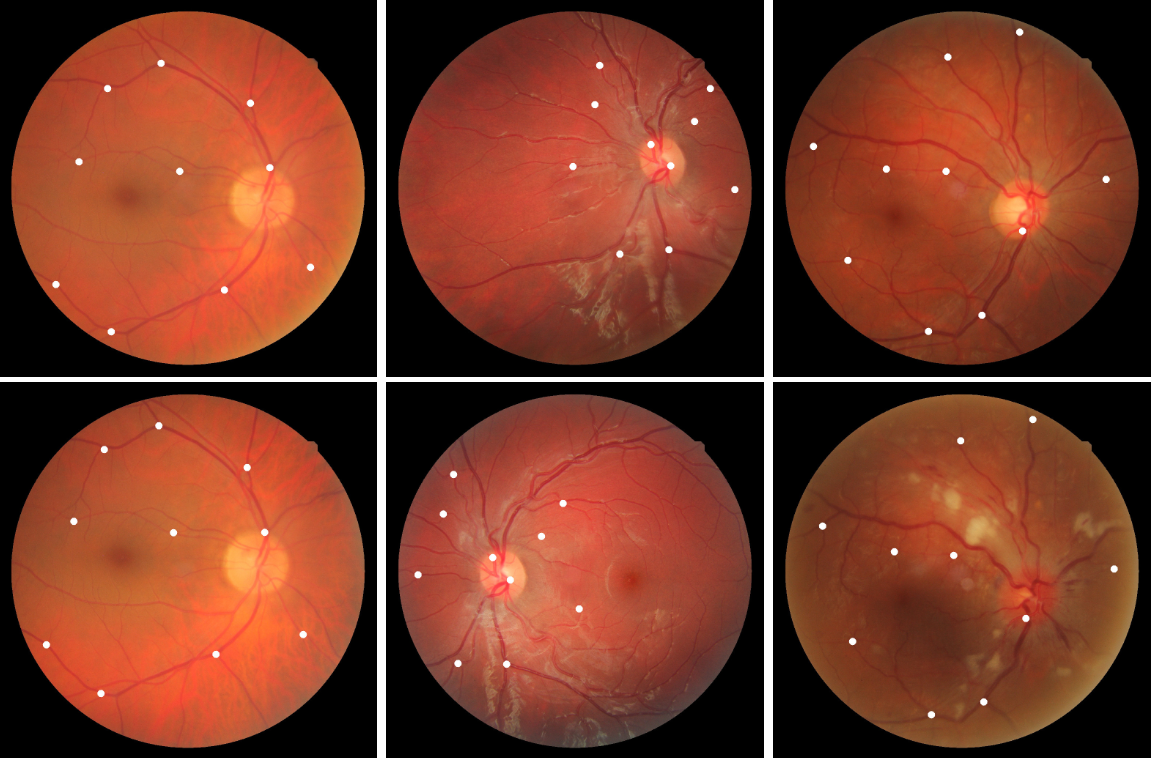
\includegraphics[width=0.8\textwidth]{imaxes/fire-ej.png}
    \caption{Exemplo de imaxes do conxunto de datos FIRE \cite{FIRE} cos puntos de control indicados. De esquerda a dereita, categorías \textit{\textsf{S}}, \textit{\textsf{P}}, \textit{\textsf{A}} .}
    \label{fig:fire_ej}
\end{figure}

\subsection{RFMID}
\label{subsec:RFMID}

O conxunto de datos RFMiD \cite{RFMiD} proporciona 3200 imaxes de fondo de ollo en cor con resolución 1712x1712, etiquetadas según se teñen algunha anomalía ou non. 
Tamén proporciona etiquetas para 45 diferentes anomalías anotadas por expertos.

Para utilizalo neste traballo, seleccionamos unha submostra e xeramos transformacións aleatorias. Gardamos as imaxes orixinais e as transformadas así como as matrices de transformación asociadas para a posterior avaliación.
Tamén se divide entre transfomacións de cor e de xeometría.

% \dots preguntar David


\subsection{Diferencias entre os datasets}
\label{subsec:Diferencias entre os datasets}

Unha vantaxe de utilizar dous conxutos de datos diferentes é que cada un deles ten características únicas que permiten avaliar o modelo en diferentes contextos.
A principal diferencia é que RMiFD é un conxunto de datos sintético, no cal non introducimos diferenzas de cor e sempre teñen unha superposición do 100\%, polo que o único que se avalia é a capacidade do modelo para realizar os rexistros xeométricos.
Polo contrario, FIRE é un conxunto de datos real, no cal existen cambios na iluminación, contraste, superposición e demais diferencias visuais, polo que se avalía a capacidade do modelo para realizar rexistros en condicións moito máis adversas.

\section{Métodos de Avaliación}
\label{sec:Métodos de Avaliación}

A evaluación divídese en dous tipos: a avaliación cualitativa, na cal analízanse os resultados de forma visual,
 e a avaliación cuantitativa, na cal se utilizan métricas numéricas para comparar os resultados en base a un criterio obxetivo.

 Ambas avaliacións son necesarias para obter unha visión completa da calidade do rexistro, xa que a avaliación cuantitativa pode non ser suficiente para detectar problemas visuais que non se reflictan nas métricas.

 \subsection{Avaliación Cuantitativa}
 \label{subsec:Avaliación Cuantitativa}
 
 Utilizamos como método de evaluación cuantitativa o proposto por FIRE \cite{FIRE}
 xerando un gráfico onde o eixo x representa o valor do límite de erro e o eixo y mostra a porcentaxe de pares de imaxes que foron rexistrados con éxito para cada límite de erro.
 
 O error de rexistro calcúlase ca distancia media entre os puntos correspondentes na imaxe fixa e móbil (cj, rj).
 Cando o erro de rexistro entre un par de imaxes está por debaixo do límite, considérase que o rexistro foi exitoso e viceversa. Isto dá lugar a unha curva monótona e continua que reflicte a relación entre a taxa de éxito e a precisión obxectivo, evitando así a necesidade de establecer un limiar arbitrario. 
 Estes gráficos utilízanse para ilustrar a precisión do rexistro tanto para casos individuais (onde se utilizan o porcentaxe de parellas de puntos rexistrados con éxito)
  como para o conxunto completo de datos.
 
Esta métrica facilita a comparación entre distintos métodos competidores e permite seleccionar o máis axeitado segundo a precisión desexada.
 
 Mentres que FIRE xa provee os puntos de referencia para a avaliación, RFMID non o fai.
 Polo tanto, para RFMID, utilizamos o mesmo método de avaliación, pero xerándo os puntos manualmente de forma que cubran o interior da máscara da imaxe fixa (separados por 50 píxeles entre si).
 
 \begin{figure}[ht]
    \centering
    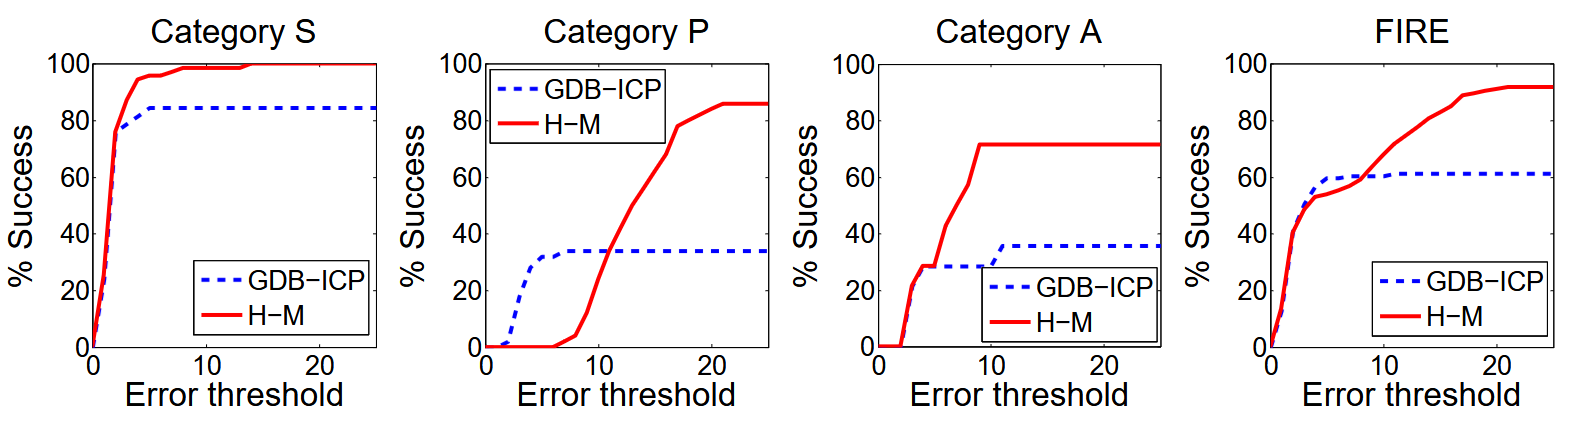
\includegraphics[width=0.8\textwidth]{imaxes/fire_aval.png}
    \caption{Gráfico de avaliación FIRE, \cite{FIRE}}
    \label{fig:fire_aval}
\end{figure}

Nalgúns casos, utilizaremos a distancia media entre os puntos correspondentes como métrica adicional para avaliar a calidade do rexistro, xa que a taxa de éxito pode non ser suficiente para detectar os cambios.

\subsection{Avaliación Cualitativa}
\label{subsec:Avaliación Cualitativa}

No caso deste traballo, a avaliación cualitativa cobra gran importancia, xa que na cuantitativa so se está a comparar sobre un número reducido de puntos en cada parexa de imaxes.
A avaliación visual permite detectar problemas que non se reflictan nas métricas cuantitativas, como artefactos visuais ou deformacións non desexadas, 
especialmente en rexistros que teñen deformacións locais que poden non coincidir con ningún punto.

No caso do dataset FIRE \cite{FIRE}, a avaliación visual é especialmente relevante, xa que tan só se proporcionan 10 puntos de referencia por imaxe, que poden non ser suficientes para avaliar a calidade do rexistro en moitas zonas da imaxe.
Xa que en RFMID \cite{RFMiD} utilízanse puntos de referencia xerados manualmente que cubren toda a imaxe, a avaliación visual é algo menos relevante, xa que é máis probable que unha deformación local incorrecta sexa detectada por algún punto e se vexa reflexado nas métricas.

\section{Proceso de Rexistro}
\label{sec:Proceso de Rexistro}

Inicializase a rede, ca arquitectura modificada nas capas de entrada e saída 
(orixinalmente [3, 256, 256, 256, 3], agora [2, 256, 256, 256, 2]) 
e o resto de parámetros relevantes (función de activación, optimizador, métrica de loss, termos de regularización, etc).

A inicialización dos pesos da rede é especialmente relevante no caso da función de activación SIREN, que é sensible a valores iniciais.
Tamén se xera un tensor de coordenadas inicial que contén todas as coordenadas dentro da máscara da imaxen fixa.

Cando comeza o adestramento por cada epoch repítese o seguinte proceso:

Mostreanse "batch size" puntos no tensor de coordenadas orixinal e estos pásanse pola rede, 
a cal devolve a transformación que predice para esas coordenadas.
A continuación, aplicase esta transformación e calculase o loss entre a imaxe móbil transformada e a imaxe fixa.
O valor de loss axústase según os termos de regularización usados, e finalmente realízase a retropropagación para actualizar os pesos da rede.

O proceso de mostraxe pode ser aleatorio ou utilizando unha estratexia específica.

Cabe destacar que a tarefa de rexistro de pulmóns é diferente da de retinografías. O tamaño das deformacións é moito maior, así como o grado de superposición entre as imaxes.
Por este motivo, non podemos asumir que os parámetros óptimos para pulmóns sexan tamén os mellores para retinas.